\setcounter{subsection}{0}
\section{CONTEXTO DEL PROYECTO}

\subsection{Antecedentes}

\textbf{Flujo y simulación de sistemas.} Un flujo describe el movimiento de entidades (vehículos, personas, paquetes de datos) por una red con restricciones de capacidad y reglas de enrutamiento. El tráfico urbano es uno de los flujos más difíciles de modelar, porque combina infraestructura (vías, intersecciones, semáforos), comportamiento humano heterogéneo, varios tipos de agentes y una demanda que cambia en el tiempo y el espacio. La simulación permite estudiar su dinámica de forma controlada y se clasifica por su nivel de detalle: la \textit{microscópica} modela cada vehículo con su posición, velocidad y comportamiento; la \textit{mesoscópica} mueve paquetes de vehículos por colas; y la \textit{macroscópica} trata el tráfico como un fluido descrito por densidad, velocidad y flujo \cite{lighthill,daganzo}.

\textbf{Matrices origen–destino y zonas de análisis.} Una matriz origen–destino (O/D) tiene en cada celda $O_{ij}$ el número de viajes de la zona $i$ a la zona $j$ en un periodo. Las zonas de análisis de tráfico (TAZ) son las unidades espaciales que agrupan áreas con movilidad homogénea. Construir una matriz desde una encuesta exige aplicar factores de expansión muestral para inferir el comportamiento de toda la población \cite{ortuzar}. En este proyecto cada viaje de la encuesta se replica $\mathrm{round}(f_{exp})$ veces, con un tope de 50 copias por registro.

\textbf{SUMO.} SUMO es un simulador microscópico de código abierto \cite{behrisch_et_al_sumo_overview_2011,krajzewicz2012}. Modela vehículos, peatones, transporte público y semáforos, importa redes de OpenStreetMap y expone la API TraCI para controlarlo en vivo. Usa por defecto el modelo de seguimiento de Krauss y un modelo de cambio de carril propio; ambos se parametrizan por tipo de vehículo (\texttt{vType}), lo que permite representar conductores heterogéneos. El proyecto usa tres de sus herramientas: \texttt{netconvert} (red), \texttt{duarouter} (rutas) y \texttt{sumo} (simulación).

\textbf{Control semafórico y seguridad.} Un semáforo reparte el derecho de paso entre los movimientos de un cruce mediante un programa de fases. El método de Webster \cite{webster} estima el ciclo que minimiza la demora media:
\begin{equation}
C_0 = \frac{1{,}5\,L + 5}{1 - Y},
\end{equation}
donde $L$ es el tiempo perdido por ciclo y $Y$ la suma de las razones flujo/flujo de saturación de los movimientos críticos. Instalar un semáforo no siempre mejora un cruce: reduce los conflictos transversales, pero puede aumentar demoras y colas. Para evaluar la seguridad sin esperar a que ocurran choques se usan medidas sustitutas de seguridad \cite{gettman}: el TTC (tiempo a la colisión, crítico por debajo de 1,5 s), el DRAC (desaceleración requerida para evitar la colisión, fuerte por encima de 3,35 m/s$^2$) y el PET (tiempo posterior a la invasión, peligroso por debajo de 1,5 s).

\textbf{Validación de modelos de tráfico.} Un modelo microscópico se valida comparando sus flujos con aforos reales. El estadístico GEH combina diferencia absoluta y relativa; el criterio habitual es GEH $<5$ en al menos 85\,\% de los puntos. En este proyecto ese criterio quedó definido, pero no pudo aplicarse (sección~\ref{sec:limitaciones-resultados}).

\textbf{La movilidad en Bogotá y Usaquén.} Bogotá combina TransMilenio (BRT), el SITP, transporte privado, bicicleta, taxis y plataformas, con una alta dependencia del vehículo particular y una oferta vial limitada por la topografía y la urbanización histórica. La localidad de Usaquén tiene 9 UTAM y 89 ZAT. La Encuesta de Movilidad 2023 registra 100.174 viajes en Bogotá; 9.341 tocan Usaquén y 2.648 tienen origen y destino dentro de la localidad. La red de OpenStreetMap de Usaquén tiene una cobertura de atributos baja (\texttt{maxspeed} 23,2\,\%, \texttt{lanes} 27,8\,\%, \texttt{name} 41,9\,\%) y la UTAM Paseo de los Libertadores es la de menor cobertura muestral (44,4\,\%).

\begin{figure}[H]
\centering
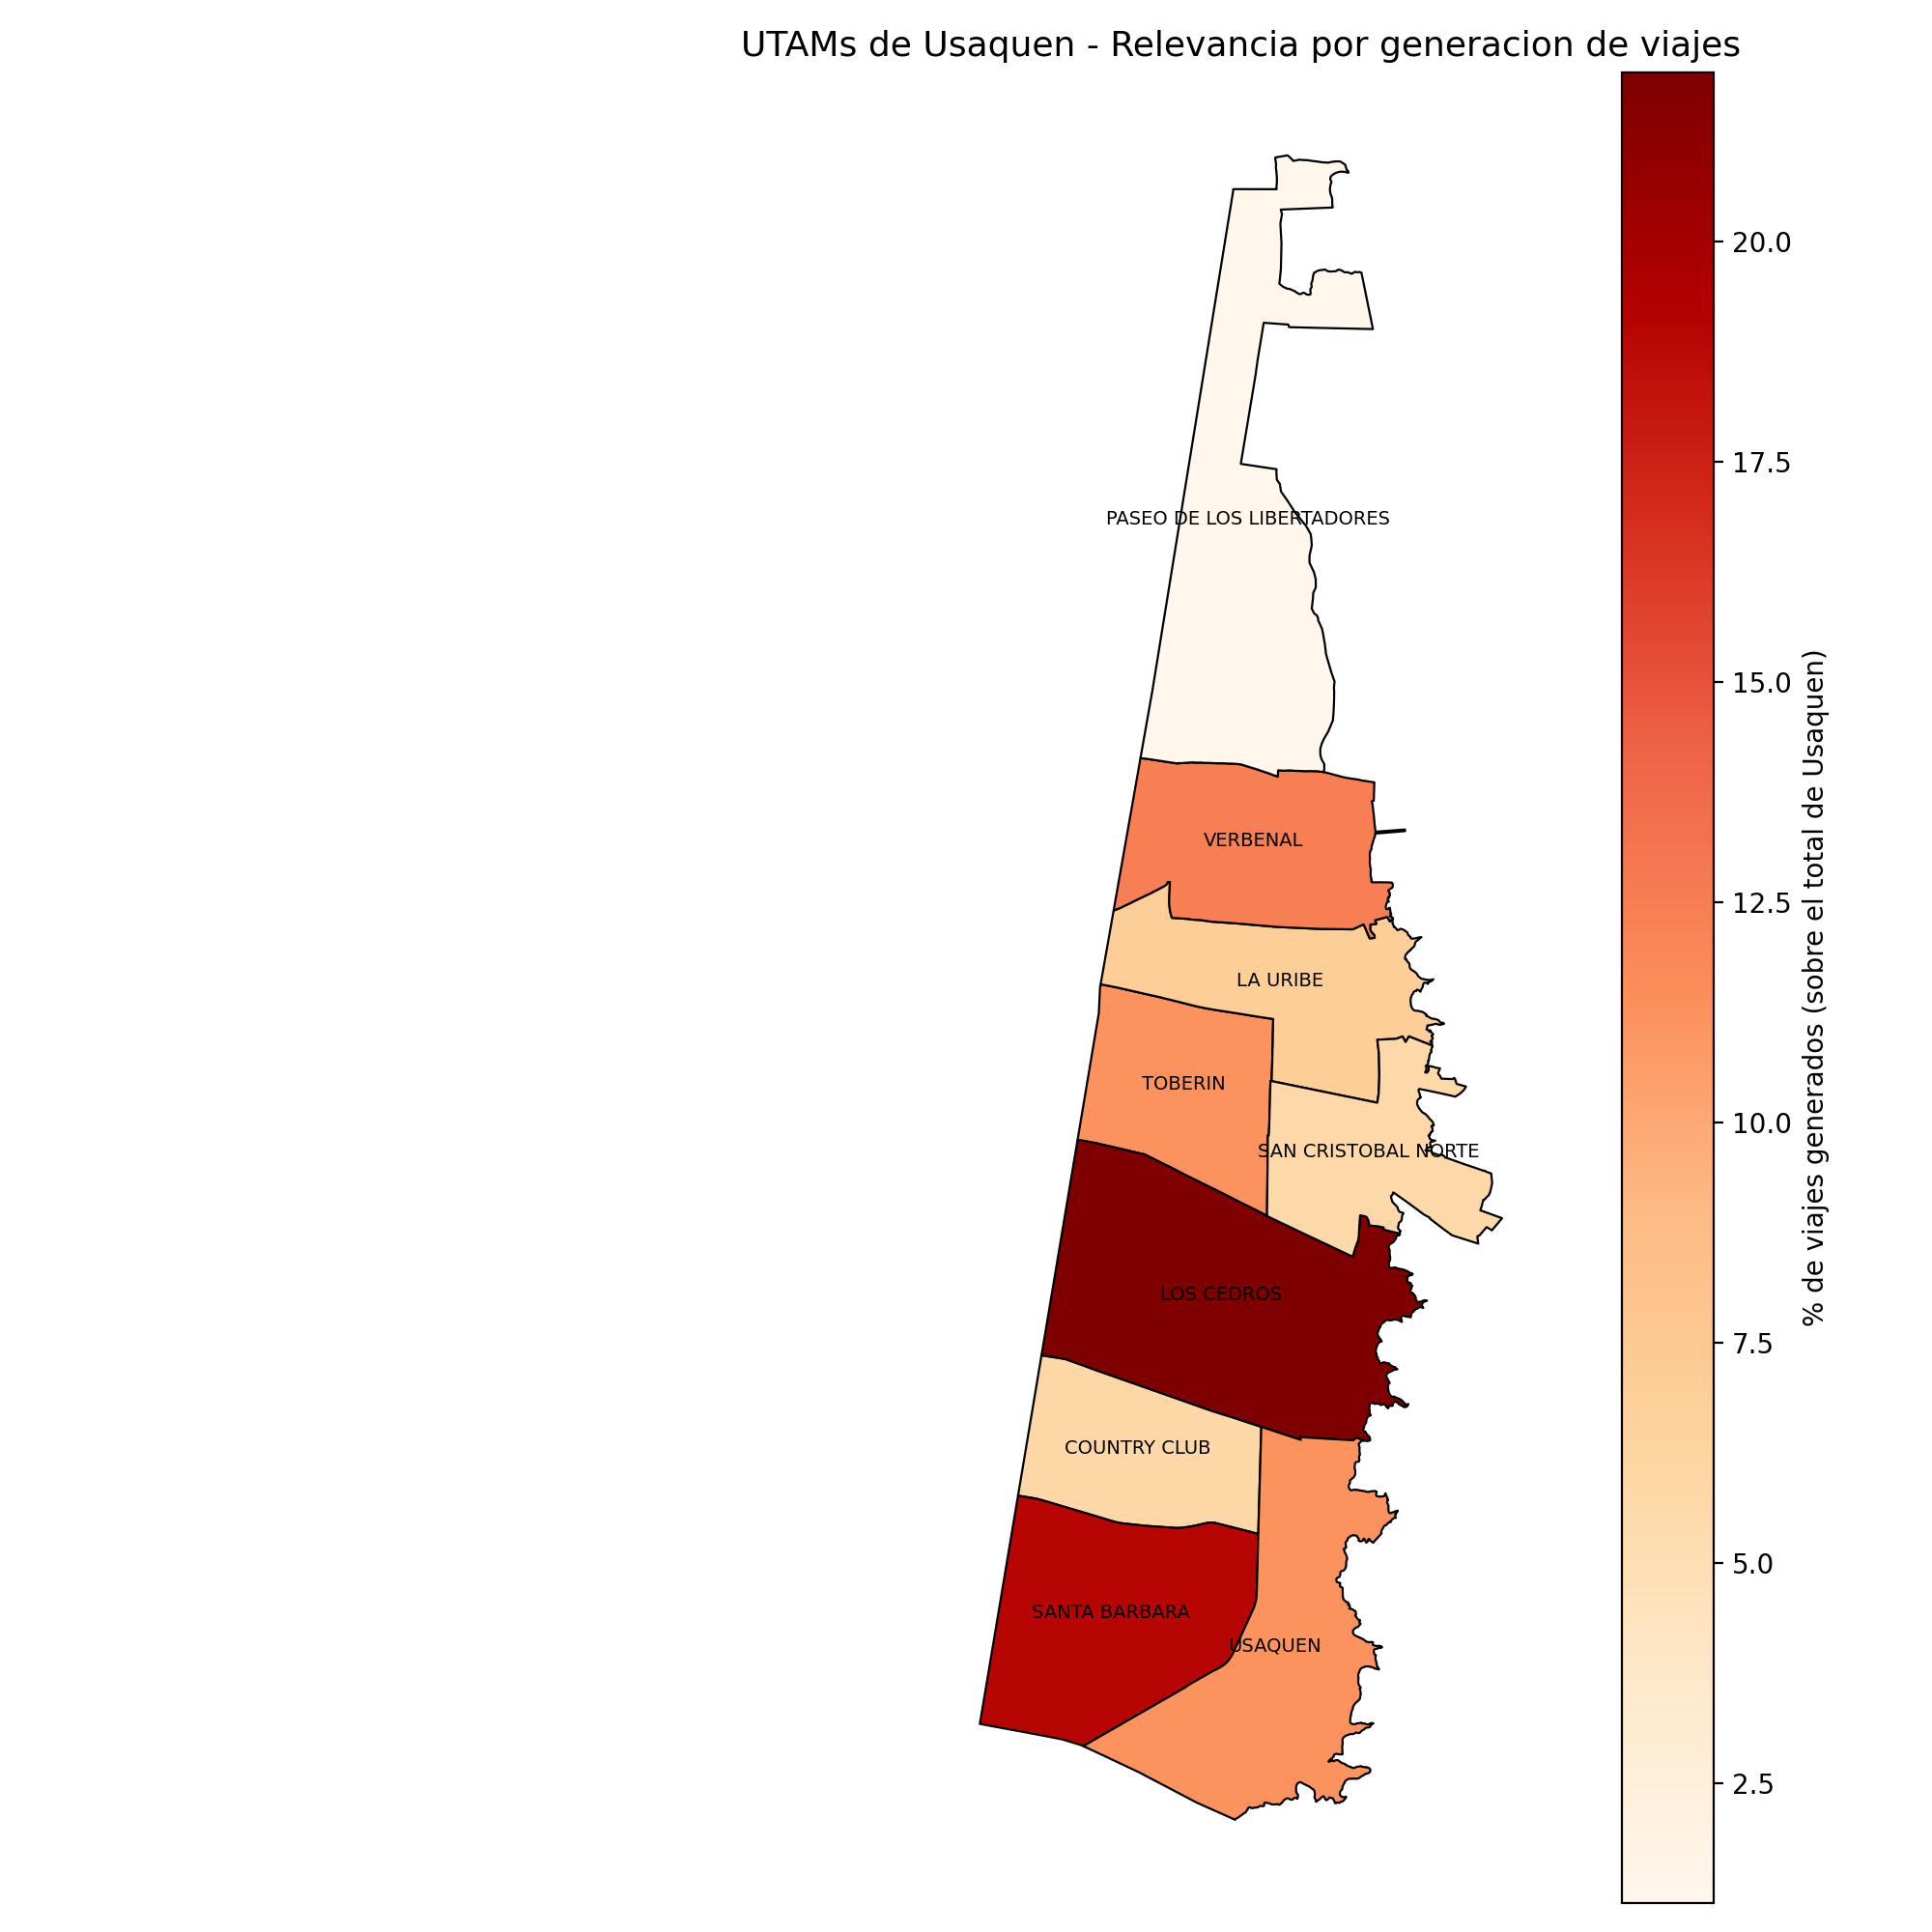
\includegraphics[width=0.6\textwidth]{mapa_utam_usaquen.png}
\caption{Unidades territoriales (UTAM) de la localidad de Usaquén.}
\label{fig:utam}
\end{figure}

\subsection{Análisis del Contexto}
\label{sec:alternativas}

\textbf{Enfoques alternativos.} El mismo problema admite cuatro enfoques distintos a la simulación con SUMO. Los \textit{modelos analíticos y la teoría de colas} son transparentes y baratos, pero exigen simplificaciones fuertes que reducen su validez en un contexto heterogéneo como el bogotano, y no permiten cambiar la red sin reformular las ecuaciones. El \textit{aprendizaje automático predictivo} \cite{vlahogianni} aprende patrones de congestión de datos históricos, pero no puede explorar escenarios que nunca ocurrieron y en Bogotá faltan series históricas estructuradas. Las \textit{APIs de tráfico en tiempo real} (Waze, Google Maps) dependen de contratos comerciales y solo describen lo que ya pasó. El \textit{modelo de cuatro pasos} \cite{mcnally} usa directamente las encuestas, pero opera por zonas y produce resultados estáticos, sin dinámica temporal ni comportamiento individual. La tabla~\ref{tab:comparacion} los compara.

\begin{table}[ht]
\renewcommand{\arraystretch}{1.15}
\centering
\small
\begin{tabular}{|p{2.9cm}|p{2.6cm}|p{2.5cm}|p{2.5cm}|p{2.4cm}|}
\hline
\textbf{Criterio} & \textbf{Simulación SUMO (propuesta)} & \textbf{Analíticos} & \textbf{ML predictivo} & \textbf{4 pasos} \\ \hline
Resolución & Microscópica & Macroscópica & Según modelo & Zonal \\ \hline
Escenarios hipotéticos & Alta & Media & Baja & Media \\ \hline
Reproducibilidad & Alta & Alta & Media & Alta \\ \hline
Datos privados & No & No & Parcial & No \\ \hline
Costo & Bajo & Bajo & Medio-alto & Alto \\ \hline
Multimodalidad & Integrada & Limitada & Si hay datos & Por etapas \\ \hline
Comportamiento individual & Sí & No & No & No \\ \hline
Aplicabilidad a Bogotá & Alta & Media & Media & Alta \\ \hline
\end{tabular}
\caption{Comparación de enfoques de solución.}
\label{tab:comparacion}
\end{table}

\textbf{Soluciones relacionadas.} Existen escenarios de SUMO construidos con datos reales, como el de Mónaco (\textit{MoST}) \cite{codeca_harri_lust_2017,codeca_harri_most_2018}, pero son escenarios únicos, elaborados con mucho trabajo manual para una ciudad concreta, y no un proceso reutilizable que parta de una encuesta de movilidad. En Colombia, Foxway \cite{10554_16495} permitió visualizar datos históricos del tráfico de Bogotá, pero no simula escenarios hipotéticos. En la literatura de automatización de simulaciones \cite{6465286,6301221} se proponen marcos genéricos de experimentación, no pipelines específicos de movilidad urbana. Para la semaforización, el proyecto \textit{Semáforos de Barranquilla} propone priorizar cruces sin semáforo con reglas duras y evidencia (siniestros, colegios, centros de salud, tramos largos sin señal); este trabajo adaptó esa lógica a Bogotá, sin su componente de modelo de lenguaje, y la acopló a una simulación microscópica con vista 3D.

\textbf{Aporte frente a lo existente.} Frente a las alternativas, la solución (i) usa solo datos públicos y herramientas abiertas, (ii) conserva el comportamiento individual de vehículos y peatones, (iii) permite preguntar «¿qué pasaría si...?» sin editar XML y (iv) es reproducible: una misma semilla y los mismos insumos producen la misma salida. Como contrapartida, es más pesada computacionalmente que un modelo analítico (una corrida completa tarda unos 12 minutos) y su calidad depende de la calidad de los datos de entrada.
